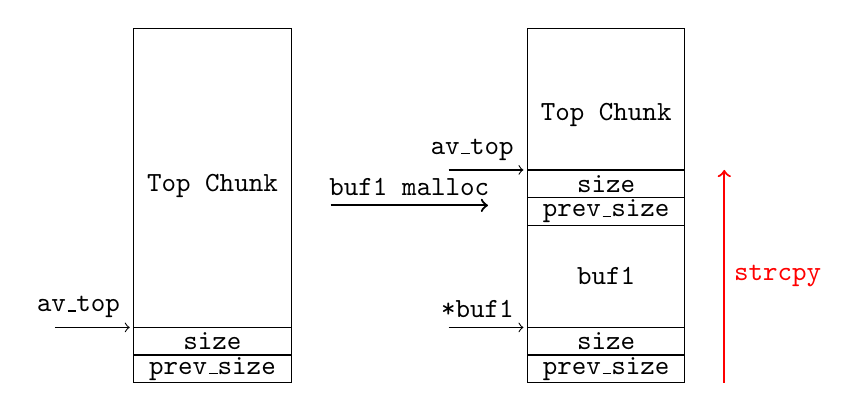
\begin{tikzpicture}[scale=0.5]
    % Draw the main rectangle
    \draw (0,0) rectangle (4,9);
    
    % Draw the divisions
    \draw (0,0.7) -- (4,0.7); % Bottom small section
    \draw (0,1.4) -- (4,1.4); % Middle small section
    
    % Labels
    \node at (2,5) {\texttt{Top Chunk}}; % Large section label
    \node at (2,1.05) {\texttt{size}}; % Middle small section label
    \node at (2,0.35) {\texttt{prev\_size}}; % Bottom small section label
    
    \draw[->] (-2,1.4) -- (-0.1,1.4);
    \node[above left] at (-0.1,1.4) {\texttt{av\_top}};
    
    \draw[thick, ->] (5,4.5) -- (9,4.5);
    \node[above] at (7,4.5) {\texttt{buf1 malloc}};
    
    % Draw the main rectangle
    \draw (10,0) rectangle (14,9);
    
    % Draw the divisions
    \draw (10,0.7) -- (14,0.7); % Bottom small section
    \draw (10,1.4) -- (14,1.4); % Middle small section
    
    \draw (10,4) -- (14,4); 
    \node at (12,2.7) {\texttt{buf1}};
    
    \node at (12,1.05) {\texttt{size}}; % Middle small section label
    \node at (12,0.35) {\texttt{prev\_size}}; % Bottom small section label
    
    \draw (10,4.7) -- (14,4.7); % Bottom small section
    \draw (10,5.4) -- (14,5.4); % Middle small section
    
    \node at (12,5.05) {\texttt{size}}; % Middle small section label
    \node at (12,4.35) {\texttt{prev\_size}}; % Bottom small section label
    
    \node at (12,6.8) {\texttt{Top Chunk}};
    
    \draw[->] (8,1.4) -- (9.9,1.4);
    \node[above left] at (9.9,1.4) {\texttt{*buf1}};
    
    \draw[->] (8,5.4) -- (9.9,5.4);
    \node[above left] at (9.9,5.4) {\texttt{av\_top}};
    
    \draw[red, thick, ->] (15,0) -- (15,5.4);
    \node[red, right] at (15,2.7) {\texttt{strcpy}};
\end{tikzpicture}